\chapter{Methodology}

This paper is based on the ideas of the AlphaZero framework applied to the game of Damath. Damath is a two-player board game combining the Filipino Checkers ``Dama'' and Mathematics. Each piece has a corresponding number and every  white square on the board has a mathematical operation. The researchers implemented the AlphaZero framework as a cycle of three stages. The researchers first generates data through self-play using the modified Monte-Carlo Tree Search algorithm of AlphaZero. Afterwards, the model is trained on the data generated from self-play. Finally, the current version of the model is evaluated against the previous model through competition.

\section{Damath}

Damath is a modified game of checkers in which the game is played on an $8 \times 8$ board with interchanging black and white tiles. There are 12 white and 12 black playing pieces that are coin-like shaped and each has a corresponding number. Each player has their pieces arranged on the white squares of the first three rows closest to them as shown in Figure \ref{fig:initial_state}. The game is always started by the player with black figures and is continued by the opponent. Regular game figures can only move diagonally on black squares towards opponent's side one at a time.

\begin{figure}
    \centering
    \includegraphics[width=0.5\linewidth]{images/initial_state.png}
    \caption{Initial State of Damath}
    \label{fig:initial_state}
\end{figure}

If there is an opponent's figure in the path of the move and the square behind that figure is vacant, the player must capture the opponent's figure by jumping over it and removing it from the playing board. The capturing figure must perform a calculation based on the mathematical operator where the capturing figure lands. If multiple such successive captures exist, the player must perform them all in one move. The result of the calculation is added to the score of the player who captured the piece.

If the player reaches opponent’s side of the board, the player's figure turns into a dama and hence has the ability to move diagonally forward and backward. Game is won if the opponent has no figures left on the board or is out of possible legal moves. The game ends in a draw if no pieces have been captured in the last 40 moves.

\clearpage

\subsection{State Representation}

A player is represented as an enum in C++ as shown in Listing \ref{lst:player_representation}.

\begin{listing}[htb]
\begin{minted}[fontsize=\footnotesize]{cpp}
enum class Player : std::int8_t {
    First = 1;
    Invalid = 0;
    Second = -1;
}
\end{minted}
\caption{Player Representation of Damath}
\label{lst:player_representation}
\end{listing}

The board is a struct containing an $8 \times 8$ matrix of piece data as shown in Listing \ref{lst:board_representation}.

\begin{listing}[htb]
\begin{minted}[fontsize=\footnotesize]{cpp}
struct Board {
    enum class Type: std::int8_t {
        Promoted = 2;
        Normal = 1;
        EnemyPromoted = -2;
        EnemyNormal = -1;
        Empty = 0;
    };
    
    struct Piece {
        Type piece_type;    
        double value;
    };

    std::array<Piece, 8 * 8> data;
};
\end{minted}
\caption{Board Representation of Damath}
\label{lst:board_representation}
\end{listing}

The state is represented as a struct containing the board and player of the current state as shown in Listing \ref{lst:state_representation}.

\begin{listing}[htb]
\begin{minted}[fontsize=\footnotesize]{cpp}
struct State {
  Board board;
  Player player;
};
\end{minted}
\caption{State Representation of Damath}
\label{lst:state_representation}
\end{listing}

\clearpage

\subsection{Action Representation}

An action is an index to the action space of Damath as shown in Listing \ref{lst:action_representation}.

\begin{listing}[htb]
\begin{minted}[fontsize=\footnotesize]{cpp}
using Action = std::int32_t;
using ActionSpace = torch::Tensor;
\end{minted}
\caption{Action Representation of Damath}
\label{lst:action_representation}
\end{listing}

The action space of Damath is represented as a $12 \times 4 \times 7$ tensor as shown in Figure \ref{fig:action_space}.

\begin{figure}[htb]
    \centering
    
\includegraphics[width=0.7\linewidth]{images/action_space.png}
    \caption{Action Space of Damath}
    \label{fig:action_space}
\end{figure}

The first dimension of the action space with a size of 12 represents one of the 12 playable pieces of the current player taking an action. The second dimension of the action space with a size of 4 represents one of the four directions on which the current piece is moving towards to. The four directions are upper left, upper right, lower left, and lower right. The last dimension of the action space represents the number of tiles the current piece is jumping over.

\subsection{Game Implementation}

This paper implemented Damath in C++ as a collection of pure functions defined by the interface shown in Listing \ref{lst:game_interface}.

\begin{listing}[htb]
\begin{minted}[fontsize=\footnotesize]{cpp}
struct Damath {
  auto initial_state() -> State;

  auto apply_action(const State& state, Action action) -> State;

  auto legal_actions(const State& state) -> std::vector<Action>;

  auto terminal_value(const State& state, Action action) -> std::optional<double>;

  auto encode_state(const State& state) -> torch::Tensor;
};
\end{minted}
\caption{Game Interface of Damath}



\label{lst:game_interface}
\end{listing}


\section{AlphaZero Framework}
The AlphaZero framework is a general reinforcement learning algorithm by \cite{silver2017masteringchessshogiselfplay} that has shown success in conquering sequential games such as chess, go, and shogi. This framework can be applied to any sequential games with perfect information. This framework has three major components: the Monte-Carlo Tree Search Algorithm, a deep neural network, and reinforcement learning through self-play.

\section{Neural Network}

The Neural Networkis a model $f_\theta(s) = (p,v)$ that takes in the state of the board denoted by $s$ and outputs $(p,v)$ where $p$ represents the policy vector which represents the probability distribution of all the moves and $v \in [-1, 1]$ which represents the predicted outcome of the state $s$.


\subsection{Monte-Carlo Tree Search Algorithm}


According to \cite{silver2017masteringchessshogiselfplay}, AlphaZero uses a general-purpose Monte-Carlo tree search (MCTS) algorithm. Each search consists of a series of simulated games of self-play that traverse a game tree from root $s_{root}$ to leaf. Each simulation proceeds by selecting in each state $s$ a move $a$ with low visit count $N(s, a)$, high move probability $P(s,a)$ and high value $Q(s, a)$ according to the current neural network $f_\theta$. The search returns a vector $\pi$ representing a probability distribution over moves, either proportionally or greedily with respect to the visit counts at the root state.

Each state-action pair $(s,a)$ stores a set of statistics, $\{N(s, a), W(s, a), Q(s, a), P(s, a)\}$, where $N(s, a)$ is the visit count, $W(s, a)$ is the total action-value, $Q(s, a)$ is the mean action-value, and $P(s, a)$ is the prior probability of selecting $a$ in $s$, as shown in Figure \ref{fig:game-tree-with-stats}.

\begin{figure}[htb]
    \centering
    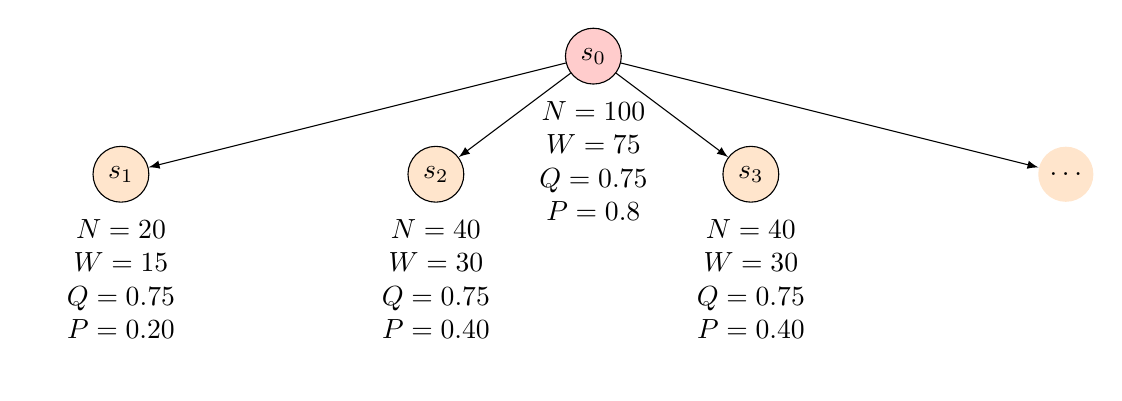
\begin{tikzpicture}[
      level 1/.style={sibling distance=40mm},
      level 2/.style={sibling distance=20mm},
      edge from parent/.style={draw,-latex},
      every node/.style={circle,draw,minimum size=7mm},
      label/.style={below=4pt, draw=none, fill=none, align=center}
      ]
      \node[label] {$N = 100$\\$W = 75$\\$Q = 0.75$\\$P = 0.8$} node[fill=red!20] {$s_0$}
        child {node[fill=orange!20] {$s_1$} node[label] {$N = 20$\\$W = 15$\\$Q = 0.75$\\$P = 0.20$}}
        child {node[fill=orange!20] {$s_2$} node[label] {$N = 40$\\$W = 30$\\$Q = 0.75$\\$P = 0.40$}}
        child {node[fill=orange!20] {$s_3$} node[label] {$N = 40$\\$W = 30$\\$Q = 0.75$\\$P = 0.40$}}
        child {node[fill=orange!20, draw=none] {$\dots$}};
    \end{tikzpicture}
    \caption{State-Action Pairs Storing a Set of Statistics}
    \label{fig:game-tree-with-stats}
\end{figure}

Each simulation begins at the root node of the search tree, $s_0$, and finishes when the simulation reaches a leaf node $s_L$ at time-step $L$, as shown in Figure \ref{fig:root-to-leaf}.

\begin{figure}[htb]
    \centering
    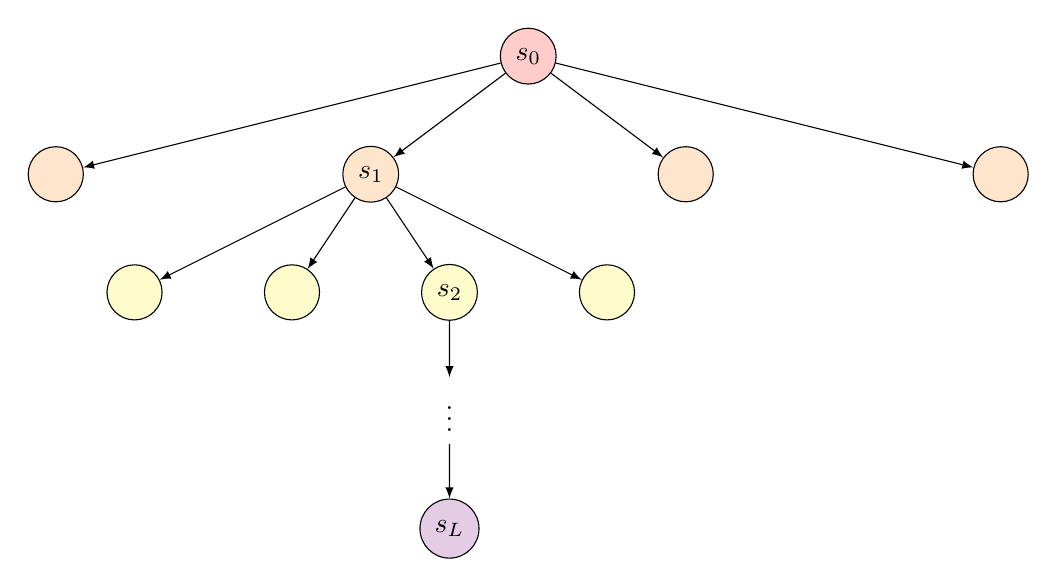
\begin{tikzpicture}[
      level 1/.style={sibling distance=40mm},
      level 2/.style={sibling distance=20mm},
      edge from parent/.style={draw,-latex},
      every node/.style={circle,draw,minimum size=7mm},
      label/.style={below=4pt, draw=none, fill=none, align=center}
      ]
      \node[fill=red!20] {$s_0$}
        child {node[fill=orange!20] {}}
        child {node[fill=orange!20] {$s_1$}
            child {node[fill=yellow!20] {}}
            child {node[fill=yellow!20] {}}
            child {node[fill=yellow!20] {$s_2$}
                child {node[draw=none] {$\vdots$}
                    child {node[fill=violet!20] {$s_L$}}}}
            child {node[fill=yellow!20] {}}}
        child {node[fill=orange!20] {}}
        child {node[fill=orange!20] {}};
    \end{tikzpicture}
    \caption{Simulation of MCTS on the Search Tree}
    \label{fig:root-to-leaf}
\end{figure}

At each of these time-steps, $t < L$, an action is selected $a_t = \operatorname{arg} \operatorname{max}_a \big(Q(s_t, a_t) + U(s_t, a_t)\big)$, using a variant of the Predictor + Upper-Confidence Bound Applied to Trees (PUCT) algorithm, $U(s, a) =  C(s) P(s, a) \sqrt{N(s)} / (1 + N(s, a))$, where $N(s)$ is the parent visit count and $C(s)$ is the exploration rate, which grows slowly with search time, $C(s) = \log\left((1 + N(s) + c_{base}) / c_{init}\right) + c_{init}$, but is essentially constant during the fast training games. The leaf node $s_L$ is added to a queue for neural network evaluation, $(\mathbf{p}, v) = f_\theta(s)$. The leaf node is expanded and each state-action pair $(s_L, a)$ is initialized to $\{N(s_L, a) = 0, W(s_L, a) = 0, Q(s_L, a) = 0, P(s_L, a) = p_a\}$. The visit counts and values are then updated in a backward pass through each step $t \leq L$, $N(s_t, a_t) = N(s_t, a_t) + 1$, $W(s_t, a_t) = W(s_t, a_t) + v$, $Q(s_t, a_t) = W(s_t,a_t) / N(s_t,a_t)$.

The modified Monte-Carlo Tree Search algorithm used in this paper is adapted from the AlphaZero framework. Internally, the node is represented as struct containing the current state and the action taken to get to this node, the index to its parent and the indices of its children, the prior policy of the node from the network, and the value and the number of visits of the node as shown in Listing \ref{lst:mcts_node}.

\begin{listing}[htb]
\begin{minted}[fontsize=\footnotesize]{cpp}
struct Node {
  using ID = std::int32_t;

  State state;
  Action action;

  Node::ID parent;
  std::vector<Node::ID> children;

  double prior = 0.0;
  double value = 0.0;
  double visits = 0.0;
};
\end{minted}
\caption{Node Representation for the Monte-Carlo Tree Search Algorithm}
\label{lst:mcts_node}
\end{listing}

The pseudocode for the modified Monte-Carlo Tree Search algorithm is shown in Algorithm \ref{alg:mcts}.

\begin{algorithm}[htb]
    \begin{algorithmic}[1]
        \Function{search}{state, model, simulations}
            \State root $\gets$ Node(state)
            \ForAll{$n \in \{1, 2,3, \ldots, \text{simulations}\}$}
                \State node $\gets$ root
        
                \Call{select}{node}
        
                \State optional\_terminal\_value $\gets$ game.terminal\_value(node.state, node.action)
                
                \If{optional\_terminal\_value.has\_value()}
                    \State value $\gets$ optional\_terminal\_value.value()
                \Else
                    \State value $\gets$ \Call{expand}{node, model}
                \EndIf
        
                \State \Call{backpropagate}{node, value}
            \EndFor

            \LComment{Action probability is proportional to child visits/}
            \State probs $\gets$ zero\_array(game.action\_size)
            \ForAll{i, child $\in$ root.children}
                \State probs[i] = child.visits
            \EndFor
            \State \Return probs / probs.sum()
        \EndFunction
    \end{algorithmic}
    \caption{Monte-Carlo Tree Search Algorithm}
    \label{alg:mcts}
\end{algorithm}

\clearpage

The pseudocode for \verb|select| function used in the modified Monte-Carlo Tree Search algorithm is shown in Algorithm \ref{alg:select}.

\begin{algorithm}[htb]
    \begin{algorithmic}[1]
        \Function{select}{node}
            \While{node.is\_expanded()}
                \State node $\gets$ \Call{highest\_child\_score}{node}
            \EndWhile
        \EndFunction
        
        \Function{highest\_child\_score}{node}
            \State child\_scores $\gets$ \{\}
            \ForAll{child $\in$ node.children}
                \State child\_scores.append(\Call{score}{child})
            \EndFor
            \Return \Call{max}{child\_scores}
        \EndFunction
        
        \Function{score}{node}
            \If{node.visits $>$ 0}
                \State mean $\gets \dfrac{1}{2}\cdot\left(\dfrac{ \text{node.value} }{ \text{node.visits} } + 1\right)$
                \If{node.parent.player $\neq$ node.player}
                    \State mean $\gets$ 1 $-$ mean
                \EndIf
            \Else
                \State mean $\gets$ 0
            \EndIf
            \State \Return $\text{mean} + \text{node.prior} \cdot C \cdot \dfrac{\sqrt{\text{node.parent.visits}}}{1 + \text{node.visits}}$  
        \EndFunction
    \end{algorithmic}
    \caption{Select Function for the Monte-Carlo Tree Search Algorithm}
    \label{alg:select}
\end{algorithm}

The pseudocode for \verb|expand| function used in the modified Monte-Carlo Tree Search algorithm is shown in Algorithm \ref{alg:expand}.

\begin{algorithm}[htb]
    \begin{algorithmic}[1]
        \Function{expand}{parent, model}
            \State legal\_actions $\gets$ game.legal\_actions(parent.state)
            \State policy, value $\gets$ model(game.encode\_state(parent.state))
            \State policy $\gets$ \Call{softmax}{policy}
            \State policy $\gets$ \Call{filter}{legal\_actions, policy}
            \State policy $\gets$ policy / policy.sum()
        
            \For{$i \in \{0, ..., \text{legal\_actions.size}\}$}
                \State legal\_actions $\gets$ legal\_actions[i]
                \State child\_state $\gets$ game.apply\_action(parent.state, action)
                \State prior $\gets$ policy[i]
                \State parent.children.append(Node(child\_state, action, prior))
            \EndFor
            \State \Return value
        \EndFunction
    \end{algorithmic}
    \caption{Expand Function for the Monte-Carlo Tree Search Algorithm}
    \label{alg:expand}
\end{algorithm}

The pseudocode for \verb|backpropagate| function used in the modified Monte-Carlo Tree Search algorithm is shown in Algorithm \ref{alg:backpropagate}.

\begin{algorithm}[htb]
    \begin{algorithmic}[1]
        \Function{backpropagate}{node, value}
            \While{node $\neq$ null}
                \State node.visits += 1
                \If{node.parent.state.player == node.state.player} 
                    \State node.value += value
                \Else
                    \State node.value -= value
                \EndIf
                \State node $\gets$ node.parent
            \EndWhile
        \EndFunction
    \end{algorithmic}
    \caption{Backpropagrate Function for the Monte-Carlo Tree Search Algorithm}
    \label{alg:backpropagate}
\end{algorithm}


The pseudocode for the  learning phase of the AlphaZero framework is shown in Algorithm \ref{alg:learning_phase}.

\begin{algorithm}[htb]
\begin{algorithmic}
    \Function{learn}{latest\_model, optimizer, iterations, selfplay\_iterations, training\_epochs}
        \For{$n \in \{0, \ldots, \text{iterations}\}$}
            \State memory $\gets$ \{\}

            \For{$i \in \{0, \ldots, \text{selfplay\_iterations}\}$}
                \State memory $+=$  \Call{self\_play}{latest\_model}
            \EndFor
            
            \For{$j \in \{0, \ldots, \text{training\_epochs}\}$}
                \State \Call{train}{latest\_model, memory, optimizer}
            \EndFor
        \EndFor
    \EndFunction
    \caption{Pseudocode for the Learning Phase of the AlphaZero Framework}
    \label{alg:learning_phase}
\end{algorithmic}
\end{algorithm}

\subsection{Self-Play}

The pseudocode for the  self-play data generation phase of the AlphaZero framework is shown in Algorithm \ref{alg:data-generation}.

\begin{algorithm}[htb]
    \begin{algorithmic}[1]
        \Function{self\_play}{model}
            \State history $\gets$ \{\}
            \State state $\gets$ game.initial\_state()
            \Loop
                \State probs $\gets$ \Call{search}{state, model}
                \State history.append((state, probs)) 
                \State action $\gets$ \Call{sample\_distribution}{probs}
                \State new\_state $\gets$ game.apply\_action(state, action)
                \State terminal\_value $\gets$ game.terminal\_value(new\_state)
                \If{terminal\_value.has\_value()}
                    \State memory $\gets$ \{\}
                    \ForAll{(hist\_state, hist\_probs) $\in$ history}
                        \State encoded $\gets$ game.encode\_state(hist\_state)
                        \State value $\gets$ hist\_state.player == player ? terminal\_value : -terminal\_value
                        \State memory.append((encoded, value, probs))
                    \EndFor
                    \State \Return memory
                \EndIf
                \State state $\gets$ new\_state
            \EndLoop
        \EndFunction
    \end{algorithmic}
    \caption{Pseudocode for the Self-Play Data Generation Phase of the AlphaZero Framework}
    \label{alg:data-generation}
\end{algorithm}


\subsection{Training}

The model is trained on the saved action probabilities as well as the outcome of playing that move which is saved on the \lstinline{memory} variable. 
    
\begin{algorithm}[htb]
\begin{algorithmic}
    \Function{train}{latest\_model, memory, optimizer}
        \State memory.shuffle()
        \For{$n \in \{0, \ldots, \text{iterations}\}$}
            \State feature, target\_value, target\_policy $\gets$ memory.sample\_batch()
            \State out\_value, out\_policy $\gets$ latest\_model(feature)
            \State loss $\gets$ \Call{mse\_loss}{out\_value, target\_value} +
            \Call{cross\_entropy}{out\_policy, target\_policy}
            \State optimizer.zero\_grad()
            \State loss.backward()
            \State optimizer.step()
        \EndFor
    \EndFunction
    \caption{Pseudocode for the Training Phase of the AlphaZero Framework}
    \label{alg:training_phase}
\end{algorithmic}
\end{algorithm}